\documentclass[lineno]{jfm}

\usepackage{showframe}
\usepackage{subcaption}

%%%%%%%%%% additional definitions %%%%%%%%%%
\newcommand\dstar{{\delta^*}} % displacement thickness
\DeclareMathOperator{\argmax}{arg\,max}
%%%%%%%%%%%%%%%%%%%%%%%%%%%%%%%%%%%%%%%%%%%%

\lefttitle{V. Ballester Ribó, J. D. Crouch, Y. Hwang and S. J. Sherwin}
\righttitle{Journal of Fluid Mechanics}

\title{Stability and transition of flow over gapped surfaces in laminar incompressible boundary layers}

\author{Víctor Ballester Ribó\aff{1}, Jeffrey D. Crouch\aff{2}, Yongyun Hwang\aff{1} \and Spencer J. Sherwin\aff{1}}

\affiliation{\aff{1}Department of Aeronautics, Imperial College London, South Kensington, London SW7 2AZ, UK
\aff{2}The Boeing Company, P.O. Box 3707, Seattle, WA 98124-2207, USA}

\corresau{Víctor Ballester Ribó, \email{v.ballester-ribo24@imperial.ac.uk}}

\begin{document}
\maketitle

\begin{abstract}
	Surface gaps, such as panel joints and access-door seams, are unavoidable on laminar-flow surfaces and can displace boundary-layer transition far upstream of its smooth-wall location. We examine the responsible mechanisms using direct numerical simulation and global stability analysis of incompressible flow over a spanwise-uniform rectangular gap in a flat-plate boundary layer, for gap widths $w/\dstar\in(0,130]$, depths $d/\dstar\in(0,4]$ and Reynolds numbers $\Rey_\dstar\in[800,3000]$, where $\dstar$ is the displacement thickness at the gap. A classification of the long-time two-dimensional dynamics identifies three attracting states: equilibria, limit cycles and chaotic attractors. Where the equilibrium is stable, the gap-induced amplification increment $\Delta n$ of Tollmien--Schlichting (TS) waves is obtained from stochastically forced linearised simulations. The resulting contours reproduce the two limiting trends measured by \citet{jeffGaps} --- depth-controlled amplification for shallow gaps and width-controlled amplification for deep gaps --- and local stability analysis attributes them to a broadening of the unstable frequency band inside the cavity, followed downstream by the emergence of a locally stable band. Stability is lost through a supercritical Hopf bifurcation producing oscillations localised at the downstream gap edge, with period doubling providing a route to two-dimensional chaos. Deep gaps become three-dimensionally unstable before the two-dimensional equilibrium does, yet this instability saturates without breakdown. Transition at the gap instead requires a two-dimensional periodic orbit that is unstable to three-dimensional perturbations; this criterion reproduces the measured bypass boundary.
\end{abstract}

\section{Introduction}\label{sec:introduction}

Skin friction is the single largest contributor to the drag of a transport aircraft in cruise, and the extent of laminar flow over the lifting and control surfaces is what ultimately sets it. With more than one hundred thousand commercial flights operated daily worldwide \citep{flightradar24}, even a modest delay of laminar--turbulent transition translates into a substantial reduction in fuel burn and emissions, which is why natural laminar flow and laminar-flow control have remained a persistent design objective for over half a century \citep{holmes1984,joslin1998,krimmelbein2021nlf}. The difficulty is that the aerodynamic surfaces that must sustain laminar flow are also manufactured, assembled and maintained surfaces. Panel joints, access doors, control-surface seams and de-icing inserts all introduce steps, gaps and waviness whose dimensions are fixed by manufacturing tolerances rather than by aerodynamics. On a modern transport wing with a chord of several metres \citep{boeing737ng,boeing787char,airbusA320tech,flyingA350}, the laminar displacement thickness over the forward portion of the chord is $\mathcal{O}(0.1\,\mathrm{mm})$, so an assembly gap of a fraction of a millimetre is already several displacement thicknesses wide. Tightening such tolerances is expensive, and doing so without a predictive model of the aerodynamic penalty is expensive for no guaranteed benefit. Quantifying, and more importantly understanding, how a gap modifies transition is therefore a prerequisite for realistic laminar-flow design \citep{Rouviere2022Amelioration,ganlinThesis}.

Under the quiet free-stream conditions characteristic of flight, transition in a nominally two-dimensional boundary layer follows the classical route: Tollmien--Schlichting (TS) waves are excited by receptivity to environmental disturbances, amplify convectively over an extended streamwise distance, and break down nonlinearly once they reach finite amplitude \citep{boundaryLayerTheory,schmid2001stability}. For the Blasius boundary layer \citep{blasius1908grenzschichten} the primary instability is two-dimensional by Squire's theorem \citep{squire1933}, and quasi-parallel linear theory predicts its growth accurately provided that non-parallel and nonlinear corrections are accounted for \citep{vanVooren,bertolotti,reedSaric1996}; three-dimensionality enters later, through secondary instability of the finite-amplitude wave \citep{faselRist1990}, or from the outset when sweep introduces a crossflow instability \citep{3dBoundaryLayers}. Engineering practice condenses this sequence into the $e^{N}$ method \citep{smithgamberoni,vanIngen1956}, in which the amplification factor
\begin{equation}\label{eq:nfactor_intro}
	n(x)=\log\left(\frac{A(x)}{A_0}\right)
\end{equation}
is integrated from linear theory and transition is declared where $n$ reaches an empirically calibrated threshold $N$. The method is not a model of breakdown but a correlation: $N$ absorbs everything that the linear amplification does not describe, in particular the receptivity amplitude $A_0$ and the disturbance environment \citep{crouchNgKachanov2015,krimmelbein2021nlf}. This is precisely what makes it extensible. A surface imperfection that alters receptivity or adds a localised burst of amplification can be represented, to leading order, by a reduction $\Delta N$ of the critical factor relative to the smooth surface, giving the variable-$N$ formulation $N=N_0-\Delta N$ \citep{crouchKosoryginNg2006,perraudArnalKuehn2014,crouch2021predicting}. The predictive burden then rests entirely on how $\Delta N$ depends on the geometry --- and on the tacit assumption that the imperfection has not changed the transition mechanism at all.

For isolated surface steps this programme has been carried out in considerable detail. \citet{klebanoffTidstrom1972} established that a two-dimensional roughness element destabilises the boundary layer mainly through the inflectional recovery region it leaves behind, rather than through the local distortion at the element itself, and subsequent theoretical and numerical work confirmed that humps and steps may either amplify or damp TS waves depending on their height, their streamwise extent and their position relative to the neutral point \citep{nayfeh1992,worner2003,dovgal1994}. Experiments quantified the associated forward movement of transition \citep{wangGaster2005,kosoryginCrouchNg2010}, and stability calculations connected that movement to the altered amplification in the distorted mean flow behind the step \citep{edelmannRist2015,hildebrand2020}. Out of this body of work emerged step-specific $\Delta N$ correlations \citep{perraud2004,perraudArnalKuehn2014,crouchKosorygin2020} that are now standard in industrial transition prediction, together with the recognition that on swept surfaces steps interact with crossflow modes in a qualitatively different manner \citep{eppink2019,tufts2017}. A separate line of enquiry established that, at sufficiently large step heights, the separated flow behind a backward-facing step and ahead of a forward-facing step supports genuinely global, three-dimensional instabilities of the recirculation region \citep{lanzerstorferBFS,lanzerstorferFFS}, so that the step ceases to be a passive amplifier and becomes an oscillator in its own right. The step problem thus already contains, in embryo, the central question of the present work: whether an imperfection acts on the incoming instability or generates its own.

Gaps have received markedly less attention than steps, despite being at least as common and geometrically richer. A gap is not a step, nor a simple superposition of two: it is a backward-facing step and a forward-facing step coupled through a cavity of finite width, and the shear layer that separates at the upstream edge must negotiate the downstream edge before the outer boundary layer can recover. The earliest evidence came from flight testing, where \citet{nenniGluyas1966} proposed a threshold based on a gap-width Reynolds number of $15\,000$ beyond which transition moved forward significantly. \citet{sinhaGuptaOberai1982} subsequently classified the internal flow topologies of laminar cavities, distinguishing the regimes in which the separated shear layer bridges the cavity from those in which it reattaches to the floor --- a distinction later refined in the cavity literature into the open and closed classifications \citep{Zhang2005,Crook2013}. A sustained experimental programme at ONERA then mapped the threshold for transition to occur at the gap, expressing it in terms of $w/\dstar$ and $d/\dstar$ \citep{oliveBlanchard1982,seraudie2010,gentili2012,perraudSeraudie2000}, and \citet{beguetONERA} synthesised these data into a model that captures both the localised peak in $n(x)$ at the gap and the far-field increment $\Delta n_{\mathit{far}}$ downstream of it, parametrised by a width-based Reynolds number and a momentum-thickness Reynolds number. Notably, that model found the gap depth to be immaterial over the range $0.2<d/w<0.7$, whereas the compressible direct numerical simulations of \citet{zahnRist} for deep gaps, $d/w>5$, reported a non-monotonic depth dependence of $\Delta n$ that they attributed to acoustic feedback within the cavity. The two findings are not contradictory --- they probe opposite corners of the parameter space --- but their coexistence is a first indication that a single scaling cannot cover the whole $(w/\dstar,d/\dstar)$ plane.

The systematic experiments of \citet{crouchKosoryginSutanto2020} and \citet{jeffGaps} resolved this by covering $0<w/\dstar<110$ and $0<d/\dstar<11$ in a single low-turbulence facility, and they provide the empirical reference against which the present computations are assessed. In the TS-dominated regime they identified two limiting behaviours: for shallow gaps the increment follows the backward-facing-step law $\Delta N=4.4\,d/\dstar$ and is independent of the width, consistent with the step-superposition argument of \citet{crouchKosorygin2020}; for deep gaps it saturates at $\Delta N\approx0.1\,w/\dstar$ and becomes insensitive to further increases in depth. The crossover, at $d/w\approx0.023$, is interpreted as the point at which the reattachment length within the cavity ceases to be set by the depth and becomes limited by the width. Crucially, however, a region of the parameter space was found in which the measured transition movement cannot be reconciled with any TS-wave amplification at all: for $d/\dstar\gtrsim1.8$ and $w/\dstar\gtrsim19$ transition occurs at or immediately downstream of the gap, at a frequency an order of magnitude above the TS band, and the variable-$N$ description breaks down. This is a change of mechanism, not a larger value of $\Delta N$, and \citet{jeffGaps} accordingly excluded it from their correlation and labelled it bypass transition.

What that bypass mechanism is has been addressed only indirectly. \citet{mathiasMedeiros2019} performed a global stability analysis of a boundary layer over a small cavity and argued that the gap-located transition originates in an instability of the shear layer spanning the cavity, sustained by the feedback loop familiar from Rossiter's analysis of rectangular cavities, in which disturbances scattered at the downstream edge propagate back upstream and re-excite the shear layer \citep{rossiter1964}. Open cavities are indeed among the best-studied self-excited flows: they oscillate through shear-layer and wake modes \citep{GharibRoshko1987,dynandcontrol}, their two-dimensional equilibria lose stability to three-dimensional centrifugal modes localised in the recirculation region \citep{bresColonius2008,Citro2015}, and the interpretation of the resulting global modes as eigenvalues of the linearised operator about a steady base flow is by now standard \citep{sippLebedev2007,theofilis2011}. A surface gap, however, sits awkwardly between these canonical problems. It is shallower than a typical cavity and deeper than a typical step; its aspect ratio $w/d$ varies over two orders of magnitude across the relevant parameter space; and, unlike an isolated cavity in an otherwise stable stream, it is embedded in a boundary layer that is itself convectively unstable. Whether the self-excited state of the cavity and the convective TS instability of the boundary layer act independently, compete, or reinforce one another, is not determined by either literature in isolation \citep{HuerreRossi}.

This is the gap in understanding that the present work addresses, and it can be stated as a single question: \emph{what dynamical sequence connects the instability of a gap flow to the onset of three-dimensional breakdown?} The question matters because linear global instability of the steady gap flow is not, by itself, a transition criterion. An unstable eigenmode grows, saturates and may well settle onto a low-amplitude limit cycle confined to the cavity without ever disturbing the downstream boundary layer; conversely, a two-dimensional oscillation that is innocuous in a strictly two-dimensional setting may be violently unstable to spanwise perturbations. Answering the question therefore requires following the flow through the entire sequence of bifurcations --- from equilibrium, through periodic and chaotic two-dimensional states, to three-dimensional breakdown --- rather than inspecting a single spectrum or a single transition-location measurement. In the language of dynamical systems, one must identify which attractor the flow actually reaches, and whether that attractor is stable in the full three-dimensional phase space \citep{natureTurbulence,hypdroynamicsNonlinearInstabilities}.

We pursue this using direct numerical simulation and global stability analysis of the two- and three-dimensional incompressible Navier--Stokes equations over a spanwise-uniform rectangular gap, for $w/\dstar\in(0,130]$, $d/\dstar\in(0,4]$ and $\Rey_\dstar\in[800,3000]$. The work has three objectives. The first is to classify the long-time states of the two-dimensional flow throughout this parameter space. We locate the boundary at which the equilibrium loses stability, show that it does so through a supercritical Hopf bifurcation whose amplitude obeys the expected normal-form scaling, and follow the subsequent period-doubling cascade to two-dimensional chaos. The shape of this boundary is itself informative: the critical width first increases with depth, reflecting the mutual interference of the two edges, and then decreases towards the limit of two isolated steps.

The second objective is to place the TS-based description on a flow-resolved footing. For every configuration admitting a stable equilibrium, the linearised equations are driven by localised stochastic forcing upstream of the gap and integrated to a statistically stationary state, from which the amplification history $n(x)$ and the increment $\Delta n=n_{\mathrm{gap}}-n_{\mathrm{flat}}$ are extracted. This reproduces both limiting trends of \citet{jeffGaps} from first principles rather than from a fitted correlation, and local spatial stability analysis of the equilibrium profiles explains them: inside the cavity the unstable frequency band broadens, so that white-noise forcing is amplified across a wider spectrum, while downstream of wide gaps the band splits into two branches separated by a locally stable window, which accounts for the abrupt drop in $n$ and the slow recovery observed for deep gaps. The agreement matters for two reasons. It confirms that the shallow- and deep-gap trends are a property of the linear response of the incompressible gap flow, and it establishes the boundary beyond which that description must fail, namely the loss of stability of the equilibrium about which the linearisation is performed.

The third objective is to determine how three-dimensional instability interacts with the nonlinear two-dimensional dynamics. We find that deep gaps become unstable to spanwise-periodic perturbations before their two-dimensional equilibrium loses stability, so that the purely three-dimensional boundary lies at smaller widths than the two-dimensional one --- yet direct simulation shows that this instability saturates into a steady streaky state that leaves the downstream boundary layer laminar. Three-dimensional instability of the equilibrium is thus necessary neither as a description of, nor sufficient as a criterion for, breakdown. The decisive pathway is instead nonlinear and sequential: the two-dimensional Hopf bifurcation creates a self-sustained oscillation localised at the downstream edge, that periodic orbit is in turn unstable to three-dimensional perturbations, and the flow departs from it into a chaotic state that spreads into the downstream boundary layer. Where such a three-dimensionally unstable periodic orbit exists, transition occurs at the gap; where it does not --- either because no periodic orbit has yet appeared, or because the one that has is stable to spanwise perturbations --- transition reverts to the conventional TS route farther downstream. This criterion reproduces the experimental bypass boundary of \citet{jeffGaps} across the parameter space, and it explains why the boundary is traced by the two-dimensional stability curve for deep gaps and by the three-dimensional curve for shallow ones.

Taken together, these results give a unified reading of surface-gap effects. A shallow gap is a passive distortion of the mean flow that modifies the amplification of an instability it does not create, and is fully described by $\Delta n$. A sufficiently deep gap is an active dynamical element that manufactures its own disturbances and, through the three-dimensional instability of the resulting oscillation, opens a route to breakdown that is independent of the incoming TS waves. The contribution of this work is therefore not only to quantify the transition penalty of a gap, but to identify the bifurcation sequence that separates these two regimes and to supply a criterion, computable from the flow itself, for deciding which one applies.

The paper is organised as follows. Section~\ref{sec:numericalSetup} describes the governing equations, the spectral/\textit{hp}-element discretisation and the computational domain. Section~\ref{sec:globalStability} presents the equilibrium base flows, their dependence on the cavity aspect ratio, and their two- and three-dimensional global stability. Section~\ref{sec:2Ddynamics} classifies the two-dimensional attracting states, computes the TS-wave amplification increment $\Delta n$ and compares it with experiment, and characterises the Hopf bifurcation and the route to chaos. Section~\ref{sec:3Ddynamics} examines the three-dimensional instabilities and the resulting transition scenarios. Conclusions are drawn in Section~\ref{sec:conclusions}.

\section{Numerical setup}\label{sec:numericalSetup}
The incompressible Navier--Stokes equations are solved using a spectral/\textit{hp}-element formulation. In nondimensional form, the governing equations are
\begin{equation}\label{eq:ns}
	\begin{aligned}
		\partial_t \boldsymbol{u} + \boldsymbol{u} \cdot \bnabla \boldsymbol{u} & = -\bnabla p + \frac{1}{\Rey} \Delta \boldsymbol{u}, \
		\bnabla \cdot \boldsymbol{u}                                            & = 0,
	\end{aligned}
\end{equation}
where $\boldsymbol{u}=(u,v)$ or $\boldsymbol{u}=(u,v,w)$ denotes the velocity field in two or three dimensions, respectively, $p$ is the pressure, and $\Rey$ is the Reynolds number. Throughout the paper, $\boldsymbol{x}=(x,y)$ or $\boldsymbol{x}=(x,y,z)$ denotes the spatial coordinates in two or three dimensions, respectively, with $x$, $y$ and $z$ denoting the streamwise, wall-normal and spanwise directions. The equations are nondimensionalised using the free-stream velocity $u_\infty$ as the characteristic velocity and the displacement thickness $\dstar$ as the characteristic length scale. The latter is evaluated at the upstream edge of the gap for the smooth-wall reference flow. Thus,
$
	\Rey \equiv \Rey_\dstar := u_\infty \dstar/\nu
$,
where $\nu$ is the kinematic viscosity. The Reynolds number is varied in the range $\Rey \in [800,3000]$.

All simulations are performed using the \texttt{Nektar++} solver \citep{nektar}, configured with a velocity-correction scheme and a continuous Galerkin projection \citep{vcs1,vcs2}. Time integration is performed using a second-order IMEX scheme, with the nonlinear advection term treated explicitly and the viscous terms treated implicitly. Spectral vanishing viscosity is added to stabilise the numerical scheme in regions containing sharp gradients \citep{svv}.

The computational domain is rectangular, with a cavity of width $w$ and depth $d$ attached to the lower wall to model the surface gap (figure~\ref{fig:domain}). The origin, $\boldsymbol{x}=\boldsymbol{0}$, is located at the upstream edge of the gap. The domain dimensions are $h=150\dstar$, $\ell_{\mathrm{i}}=100\dstar$ and $\ell_{\mathrm{o}}=1000\dstar$, which are chosen to ensure a fully developed upstream boundary layer and to minimise the influence of the upper and downstream boundaries on the region of interest. A Blasius profile ($\boldsymbol{u}=\boldsymbol{u}_\mathrm{BL}(y)$) is prescribed at the inlet and no-slip conditions ($\boldsymbol{u}=\boldsymbol{0}$) are imposed on the solid walls. At the upper boundary, a far-field condition ($\boldsymbol{u}=\boldsymbol{u}_\infty(x)$) is imposed. At the outlet, the outflow boundary condition of \citet{dong} is used to minimise numerical instabilities when energetic vortices leave the computational domain.

\begin{figure}[ht]
	\centering
	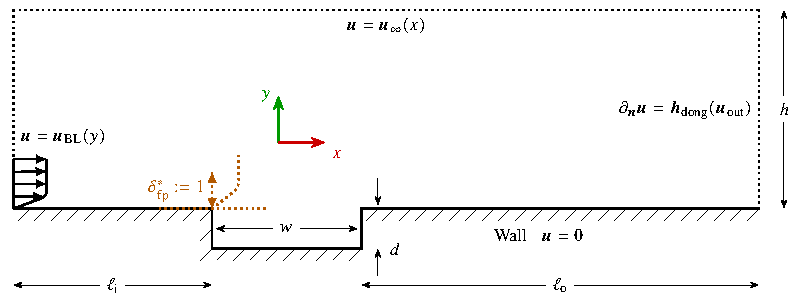
\includegraphics{Images/domainBaseflowExtended.pdf}
	\caption{Computational domain and boundary conditions for two-dimensional nonlinear simulations. Dimensions are anisotropically rescaled for clearer visualisation of the gap geometry.}
	\label{fig:domain}
\end{figure}

For the two-dimensional simulations, the domain is discretised using a structured mesh of quadrilateral elements in the boundary-layer region and unstructured triangular elements in the far field. Approximately 7000 elements are used in each simulation. A polynomial order of $p=5$ is used for the velocity field and $p=4$ for the pressure field. This choice satisfies the inf-sup condition and prevents the numerical instabilities associated with an incompatible velocity-pressure discretisation \citep[see][]{infsupCondition,infsupTaylorHood}. The polynomial basis is constructed from modified hierarchical Legendre polynomials of the corresponding dimensions \citep{spectralhpSpencerBible}. For the three-dimensional simulations, the two-dimensional mesh is extruded in the spanwise direction and periodic boundary conditions are imposed. The solution is expanded using 16 complex Fourier modes in the spanwise direction. The resulting spatial resolution is sufficient to resolve the relevant flow features, as confirmed by grid-convergence studies.

For global linear stability analysis (LSA), the Navier--Stokes equations (\ref{eq:ns}) are linearised about a base flow $\boldsymbol{U}$, which is either an equilibrium solution for classical LSA or a periodic orbit for Floquet analysis. When the base flow is an unstable equilibrium, the selective frequency damping method \citep{sfd} is used to suppress the unstable modes and obtain the equilibrium solution. The linearised equations are then solved to determine the corresponding eigenvalues and eigenmodes. They are given by
\begin{equation}\label{eq:linearizedNS}
	\begin{aligned}
		\partial_t \boldsymbol{u}' + \boldsymbol{U} \cdot \bnabla \boldsymbol{u}'
		+ \boldsymbol{u}' \cdot \bnabla \boldsymbol{U}
		                              & = -\bnabla p' + \frac{1}{\Rey}\Delta\boldsymbol{u}', \\
		\bnabla \cdot \boldsymbol{u}' & = 0.
	\end{aligned}
\end{equation}
where $\boldsymbol{u}'$ and $p'$ denote the perturbation velocity and pressure, respectively. For later reference, the linearised equations can be written in operator form as
\begin{equation}
	\partial_t \boldsymbol{u}' = \mathcal{L}(\boldsymbol{U})\boldsymbol{u}',
\end{equation}
where $\mathcal{L}(\boldsymbol{U})$ denotes the linearised Navier--Stokes operator around the base flow $\boldsymbol{U}$. For a steady base flow, solutions of (\ref{eq:linearizedNS}) are sought in Fourier space in $z$ direction and Laplace space in time using the ansatz
\begin{equation}
	\boldsymbol{u}'(x,y,z,t)
	= \hat{\boldsymbol{u}}(x,y)
	\exp\left(\mathrm{i}(\beta z-\omega t)\right),
\end{equation}
where $\hat{\boldsymbol{u}}$ is the eigenmode, $\beta$ is the spanwise wavenumber ($\beta=0$ for two-dimensional LSA), and $\omega$ is the complex temporal frequency. For a spanwise-periodic domain of length $b$, the admissible wavenumbers are $\{\beta_n = 2\pi n/b:n=0,\ldots,15\}$. For each prescribed $\beta$, substitution of the above ansatz into (\ref{eq:linearizedNS}) gives an eigenvalue problem of the form
\begin{equation}
	-\mathrm{i}\omega\hat{\boldsymbol{u}}
	= \mathcal{L}_{\beta}(\boldsymbol{U})\hat{\boldsymbol{u}},
\end{equation}
from which the eigenvalues $\omega$ and corresponding eigenmodes
$\hat{\boldsymbol{u}}$ are obtained. The linearised spatial operator $\mathcal{L}$ is discretised using the same spectral/\textit{hp}-element formulation as in the nonlinear simulations. Since the base flow $\boldsymbol{U}$ satisfies the non-homogeneous boundary conditions, the $\mathcal{L}$ is equipped with homogeneous boundary conditions of the corresponding type. The resulting eigenvalue problem is solved using a modified Arnoldi method \citep{arnoldiMethod}.
\section{Global stability analysis}\label{sec:globalStability}

\subsection{Base flows}
For sufficiently small gap depths and widths, the flow asymptotically approaches an equilibrium state, provided that the initial condition lies within basin of attraction of the equilibrium point. The equilibrium flow topology in the boundary layer outside the gap remains close to a Blasius profile, while the flow topology inside the cavity changes strongly with the cavity aspect ratio $w/d$ (figure~\ref{fig:baseflow}).

\begin{figure}[ht]
	\begin{subfigure}{0.33\linewidth}
		\centering
		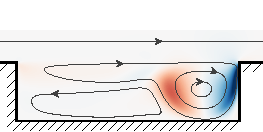
\includegraphics{Images/2dstates/pdfs/gapd4_w15.pdf}
		\caption{$w=15\dstar$, $d=4\dstar$}
		\label{fig:baseflowA}
	\end{subfigure}
	\begin{subfigure}{0.33\linewidth}
		\centering
		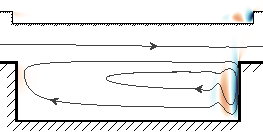
\includegraphics{Images/2dstates/pdfs/gapd1.5_w30.pdf}
		\caption{$w=30\dstar$, $d=1.5\dstar$}
		\label{fig:baseflowB}
	\end{subfigure}
	\begin{subfigure}{0.33\linewidth}
		\centering
		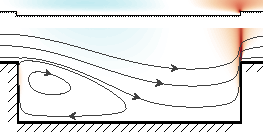
\includegraphics{Images/2dstates/pdfs/gapd1_w60.pdf}
		\caption{$w=60\dstar$, $d=1\dstar$}
		\label{fig:baseflowC}
	\end{subfigure}\\[10pt]
	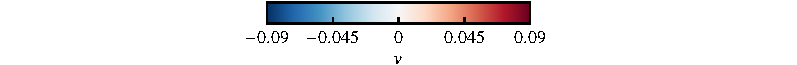
\includegraphics{Images/2dstates/pdfs/colorbar_equilibrium.pdf}
	\caption{Equilibrium solutions for three representative gap geometries shown using wall-normal-velocity contours and streamlines. All geometries are rescaled to match the aspect ratio of the first case ($w/d = 15/4$) for visual comparison; the original unscaled domain profiles are shown above the last two panels.}
	\label{fig:baseflow}
\end{figure}
For small $w/d$ (figure~\ref{fig:baseflowA}), a recirculation vortex forms within the cavity beneath the shear layer spanning the gap. This topology is characteristic of an open cavity, for which the separated shear layer remains detached from the cavity floor and the cavity interior is dominated by recirculating flow \citep{Crook2013}.

Increasing the aspect ratio to $w/d$ (figure~\ref{fig:baseflowB}) produces a more elongated, shallow recirculation region. The internal reverse flow is increasingly confined in the wall-normal direction, while the flow still features a recirculation vortex in the vicinity of the downstream edge of the gap. This evolution is consistent with the classical open-to-closed cavity transition, whereby increasing the cavity width-to-depth ratio brings the separated shear layer progressively closer to the cavity floor \citep{Zhang2005,Crook2013}.

Increasing $w/d$ further (figure~\ref{fig:baseflowC}), the cavity is very shallow and the recirculating motion is confined predominantly to a thin region adjacent to the upstream edge of the gap. In contrast to the deep-cavity case, the outer shear layer exhibits strong streamwise curvature. The resulting structure approaches the closed-cavity topology, for which the separated shear layer reattaches to the cavity floor before leaving the cavity \citep{Zhang2005}.

In the limit $w/d\to\infty$, the two cavity steps become asymptotically separated in the streamwise direction, and the flow may be interpreted locally as a backward-facing-step (BFS) flow in the vicinity of the upstream edge and a forward-facing-step (FFS) flow near the downstream edge. The shear layer separated from the upstream step extends across the gap and becomes increasingly less affected by the downstream edge. The associated recirculation remains confined near the upstream step. Near the downstream edge, the shear layer hits the wall and is deflected back into the external flow, resulting in a flow topology similar to that of a forward-facing step.

\subsection{Stability of the base flows}

To assess the stability of the equilibrium states, a biglobal stability analysis is performed for both spanwise-uniform ($\beta=0$) and spanwise-varying ($\beta\neq0$) perturbations. For spanwise-varying perturbations, the leading eigenvalue is computed for the range of spanwise wavenumbers $\beta_n$ described above, and the maximum growth rate is retained. A spanwise domain length $b=4d$ is used throughout. The stability of spanwise-varying perturbations is therefore characterised by the growth rate
\begin{equation}
	\sigma_{\mathrm{3D}}
	=
	\max_{n=1,\ldots,15}
	\max
	\big\{
	\Re(\lambda):
	\lambda\in
	\sigma(
	\mathcal{L}_{w,d,\beta_n}^{h,p,\mathrm{3D}}
	)
	\big\},
\end{equation}
where $\mathcal{L}_{w,d,\beta_n}^{h,p,\mathrm{3D}}$ denotes the discretised linear operator associated with a gap of width $w$, depth $d$, and spanwise wavenumber $\beta_n$, and $\sigma(\cdot)$ denotes the spectrum of the operator.

Similarly, the growth rate associated with spanwise-uniform (two-dimensional) perturbations is defined as
\begin{equation}
	\sigma_{\mathrm{2D}}
	=
	\max
	\big\{
	\Re(\lambda):
	\lambda\in
	\sigma(
	\mathcal{L}_{w,d}^{h,p,\mathrm{2D}}
	)
	\big\}.
\end{equation}
Here, $\mathcal{L}_{w,d}^{h,p,\mathrm{2D}}$ denotes the discretised linear operator associated with a two-dimensional domain containing a gap of width $w$ and depth $d$.

The onset of instability is determined by identifying the values of $w$ and $d$ for which $\sigma_{\mathrm{2D}}$ and $\sigma_{\mathrm{3D}}$ become positive. This procedure defines the two-dimensional and purely three-dimensional stability boundaries in the $(w/\dstar,d/\dstar)$ plane. The frequency of the leading two-dimensional mode is given by
\begin{equation}
	\omega_{\mathrm{2D}}
	=
	\Im\left(\argmax\big\{\Re(\lambda) : \lambda \in\sigma(\mathcal{L}_{w,d}^{h,p,\mathrm{2D}})\big\}\right).
\end{equation}
The corresponding definition is used for the three-dimensional modes. Figure~\ref{fig:3d2dDynamics1000} compares the resulting stability boundaries with the experimental by-pass transition boundary reported by \citet{jeffGaps} at $\Rey=1000$.

\begin{figure}[ht]
	\centering
	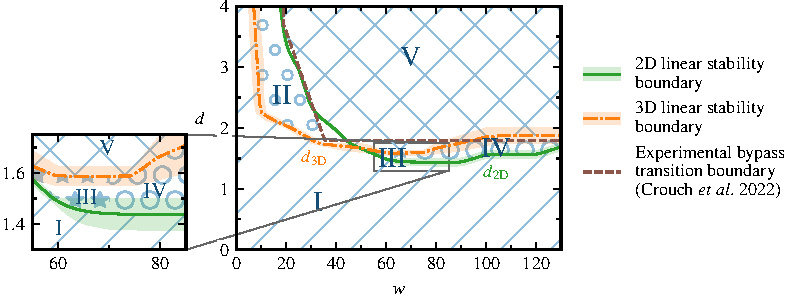
\includegraphics{Images/3d2dStabilityCurveRe1000.pdf}
	\caption{Three-dimensional and two-dimensional linear stability boundaries in the $(w/\dstar,d/\dstar)$ plane at $\Rey=1000$. Shaded bands indicate the interpolation uncertainty associated with the discrete simulation grid. The dashed brown line shows the experimental boundary beyond which transition occurs at the gap location rather than through the downstream primary instability mechanism \citep{jeffGaps}. The different regions indicate the corresponding dynamical regimes discussed in the text.}
	\label{fig:3d2dDynamics1000}
\end{figure}

For deep gaps $(d/\dstar \gtrsim 1.75)$, the purely three-dimensional stability boundary lies at smaller gap widths than the two-dimensional boundary. This indicates that spanwise disturbances can destabilize the flow before the two-dimensional equilibrium becomes unstable. For shallower gaps $(1.375 \lesssim d/\dstar \lesssim 1.75)$, the opposite behaviour is observed, with the two-dimensional instability occurring first. For deep gaps, the two-dimensional stability boundary closely follows the experimental boundary separating transition through downstream TS waves from transition initiated at the gap location reported by \citet{jeffGaps}. For shallow gaps, however, the three-dimensional stability boundary provides a closer agreement with the experimental boundary.

To describe this behaviour more precisely, the two stability boundaries are denoted by $w\mapsto d_\text{2D}(w)$ and $w\mapsto d_\text{3D}(w)$, respectively. Looking at very deep gaps $(d/\dstar \gg 50$), it has been verified that these curves are defined over intervals $\mathcal{W}_\text{2D},\mathcal{W}_\text{3D}\subset[0,\infty)$, with $\mathcal{W}_\text{2D}\subset\mathcal{W}_\text{3D}$. Within this range, the experimental by-pass transition boundary is closely described by
\begin{equation}
	w\longmapsto
	\begin{cases}
		d_\text{3D}(w),                        & w\in\mathcal{W}_\text{3D}\setminus\mathcal{W}_\text{2D}, \\
		\max\{d_\text{2D}(w),d_\text{3D}(w)\}, &
		w\in\mathcal{W}_\text{2D}\cap\mathcal{W}_\text{3D}.
	\end{cases}
\end{equation}
Global flow instability, on the other hand, occurs after crossing the boundary
\begin{equation}
	w\longmapsto
	\begin{cases}
		d_\text{3D}(w),                        & w\in\mathcal{W}_\text{3D}\setminus\mathcal{W}_\text{2D}, \\
		\min\{d_\text{2D}(w),d_\text{3D}(w)\}, &
		w\in\mathcal{W}_\text{2D}\cap\mathcal{W}_\text{3D}.
	\end{cases}
\end{equation}

The close agreement between the experimental boundary and the stability results suggests that both two- and three-dimensional instabilities play a role in bypassing the primary transition mechanism of the boundary layer (see Section~\ref{sec:3Ddynamics}).

The boundary curves in figure~\ref{fig:3d2dDynamics1000} divide the parameter space into several regions with distinct stability properties. Region I corresponds to equilibria that are stable to both two- and three-dimensional perturbations. Region II contains equilibria that are stable to two-dimensional perturbations but unstable to three-dimensional disturbances. Regions III and IV correspond to flows that are unstable to two-dimensional perturbations but remain stable to purely three-dimensional perturbations. Their different behaviour discussed in Section~\ref{sec:2Ddynamics}. Finally, region V is unstable to both two- and three-dimensional perturbations.

The two-dimensional and purely three-dimensional modes differ in both their spanwise structure and temporal behaviour. The two-dimensional mode is uniform in the spanwise direction and is associated with oscillations of the cavity shear layer. In contrast, the purely three-dimensional mode has a positive spanwise wavenumber and produces alternating streamwise structures. The real part of the most unstable modes for $(w/\dstar,d/\dstar)=(19,4)$ at $\Rey=1000$ are shown in figure~\ref{fig:modes}. The modes are visualised using isosurfaces of the streamwise velocity eigenmode $\hat{u}$.

\begin{figure}[ht]
	\centering
	\begin{subfigure}{0.495\linewidth}
		\centering
		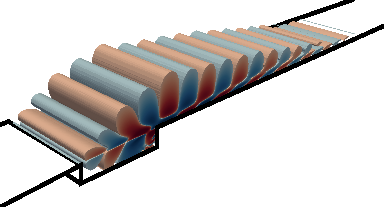
\includegraphics{Images/2D_3Dmode/pdfs/d4w19_2dmode.pdf}
		\caption{2D mode}
	\end{subfigure}
	\begin{subfigure}{0.495\linewidth}
		\centering
		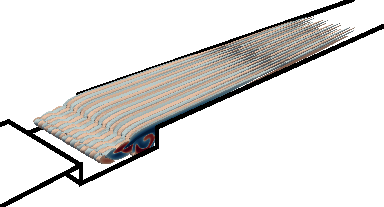
\includegraphics{Images/2D_3Dmode/pdfs/d4w19_3dmode.pdf}
		\caption{Purely 3D mode}
	\end{subfigure}\\[10pt]
	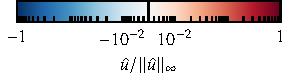
\includegraphics{Images/2D_3Dmode/pdfs/colorbar.pdf}
	\caption{Real part of the most unstable two- and purely-three-dimensional modes for the gap configuration $(w/\dstar,d/\dstar)=(19,4)$ at $\Rey=1000$. The modes are visualised using isosurfaces of the streamwise velocity eigenmode $\hat{u}$ on a two-sided logarithmic scale.}
	\label{fig:modes}
\end{figure}

The three-dimensional mode features long streamwise streaks downstream of the gap. A two-sided logarithmic scale is used to make these relatively weak streaks visible, as their amplitude is much smaller than that of the eigenmode structure inside the cavity. In contrast, the two-dimensional mode has more homogeneously distributed amplitudes across degrees of freedom near the downstream edge of the gap. For the present configuration, the frequency of the three-dimensional mode is $\omega_{\mathrm{3D}}\simeq0.0256$, compared with $\omega_{\mathrm{2D}}\simeq0.2457$ for the two-dimensional mode.

\section{Two-dimensional dynamics}\label{sec:2Ddynamics}
Building on the correspondence between the two-dimensional stability boundary and the experimental transition boundary, the nonlinear two-dimensional dynamics of flow over gapped surfaces are examined. A systematic DNS parameter sweep is performed over gap depths $d/\dstar$, gap widths $w/\dstar$, and Reynolds numbers $\Rey$. The two-dimensional dynamical regimes identified at $\Rey=1000$ are summarized in figure~\ref{fig:2Ddynamics1000}.

\begin{figure}[ht]
	\centering
	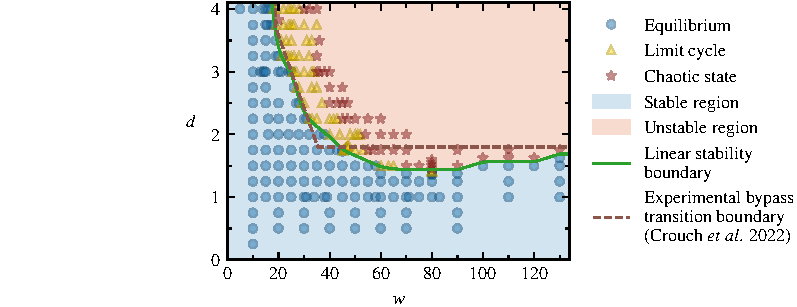
\includegraphics{Images/inc2dStabilityCurveRe1000.pdf}
	\caption{Limit set classification over the parameter space $0< w/\dstar \leq 130$ and $0 < d/\dstar \leq 4$ at $\Rey = 1000$. Blue circles denote equilibrium states, yellow triangles denote limit cycles, and red stars denote chaotic states. The continuous green line represents the linear stability boundary separating the locally stable and unstable regimes, shaded in blue and red respectively. The dashed brown line represents the experimental boundary beyond which flow transition is observed at the gap location rather than through downstream primary instability mechanisms \citep{jeffGaps}.}
	\label{fig:2Ddynamics1000}
\end{figure}
As said in the previous section, for sufficiently small gap depths and widths, the flow asymptotically approaches an equilibrium state. For sufficiently deep gaps, increasing the width leads to a series of bifurcations that eventually produce chaotic dynamics. The first bifurcation is a supercritical Hopf bifurcation, resulting in the emergence of a stable periodic orbit. Further increases in the gap width lead to the onset of chaotic dynamics. The two-dimensional transition to chaos has not been studied in detail in this work; however, several period-doubling bifurcations have been observed in the simulations (see Section~\ref{sec:bifurcations}).

The shape of the linear stability boundary also deserves attention. As the gap depth increases, the critical gap width for the onset of instability increases until reaching a maximum at an intermediate gap depth, where the interaction between the two steps is strongest. Beyond this depth, further increases in gap width have a stabilizing effect, and the system eventually approaches the asymptotic limit corresponding to two isolated steps.

\subsection{TS waves amplification (2D stable regime)}
TS waves are the dominant primary convective instability mechanism in two-dimensional laminar boundary layers \citep{schmid2001stability,boundaryLayerTheory}. However, laminar boundary layers are globally stable to two-dimensional perturbations. Therefore, a continuous source of noise is required to excite TS waves. To evaluate and corroborate the TS-wave amplification trends reported experimentally by \citet{jeffGaps}, linearized simulations are performed about the equilibrium base states $\boldsymbol{U}$ obtained from DNS (blue circles in Figure~\ref{fig:2Ddynamics1000} and regions I and II in Figure~\ref{fig:3d2dDynamics1000}). A body force $\boldsymbol{f}=(f_u,f_v)$ is added to the right-hand side of \eqref{eq:linearizedNS} to excite TS waves. The forcing has a divergence-free Gaussian spatial envelope and is driven in time by zero-mean, unit-variance Gaussian white noise, $X_t$:
\begin{align}
	f_u(\boldsymbol{x},t) & = -(y-y_{\text{c}}) \exp\big({-\alpha{|\boldsymbol{x}-\boldsymbol{x}_{\text{c}}|}^2}\big) X_t, \\
	f_v(\boldsymbol{x},t) & = (x-x_{\text{c}}) \exp\big({-\alpha{|\boldsymbol{x}-\boldsymbol{x}_{\text{c}}|}^2}\big) X_t,
\end{align}
where $\alpha = 100$, $\boldsymbol{x}_{\text{c}} =(x_{\text{c}},y_{\text{c}}) = (-95, 0.5)\dstar$, $|\cdot|$ denotes the Euclidean norm. The spatial envelope confines the forcing to a small circular region of radius approximately $0.5\dstar$ centred at $\boldsymbol{x}_{\mathrm{c}}$. Although ambient disturbances in experiments are neither strictly white nor Gaussian, this stochastic model provides a standard and reproducible representation of the external forcing.

The linearized system is integrated forward in time until the initial transient has decayed and a statistically stationary response is reached. Temporal averaging is then used to obtain the stationary root-mean-square (RMS) disturbance amplitude. Following the classical $e^n$ method \citep{smithgamberoni,vanIngen1956}, the amplitude $A(x)$ of a disturbance evolving from a reference position $x_0$ is written as
\begin{equation}
	A(x) = A(x_0) \exp\left( n_{x_0}(x) \right),
	\label{eq:amplitudeEvolution}
\end{equation}
where the corresponding local $n$-factor is
\begin{equation}
	n_{x_0}(x) = \log\left( \frac{A(x)}{A(x_0)} \right).
	\label{eq:nfactorAmplitude}
\end{equation}
For brevity, the subscript $x_0$ is omitted hereafter, such that $n(x)\equiv n_{x_0}(x)$. The disturbance amplitude is defined as the wall-normal $L^2$-norm of velocity perturbations:
\begin{equation}
	A(x) := {\||\boldsymbol{u}'|\|}_{L^2(\mathcal{Y}(x))} = {\left( \int_{\mathcal{Y}(x)} (u'^2 + v'^2) \mathrm{d}y\right)}^{1/2},
	\label{eq:amplitudeNorm}
\end{equation}
where $\mathcal{Y}(x)$ denotes the wall-normal section at streamwise location $x$. For stochastically forced simulations, the corresponding operational amplitude is the RMS value,
\begin{equation}
	A(x) := {\left( \int_{\mathcal{Y}(x)} \left\langle u'^2 + v'^2\right\rangle \mathrm{d}y\right)}^{1/2},
	\label{eq:amplitudeRMS}
\end{equation}
where $\langle \cdot \rangle$ denotes temporal expectation over the stationary stochastic ensemble. The minimum disturbance amplitude measured upstream of the gap is chosen as the reference $A(x_0)$ for constructing the $n$ curve.

\begin{figure}[ht]
	\centering
	\begin{subfigure}{0.495\linewidth}
		\centering
		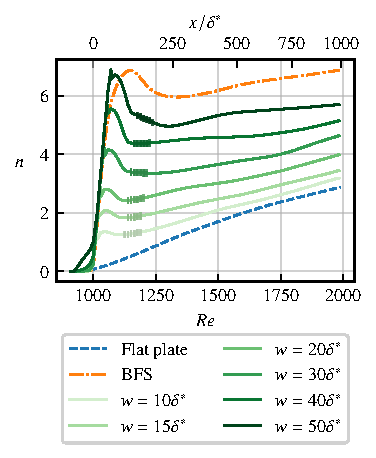
\includegraphics{Images/nfactorCurvesd1.5.pdf}
		\caption{Gaps with constant depth $d=1.5\dstar$.}
		\label{fig:nfactorCurvesA}
	\end{subfigure}
	\begin{subfigure}{0.495\linewidth}
		\centering
		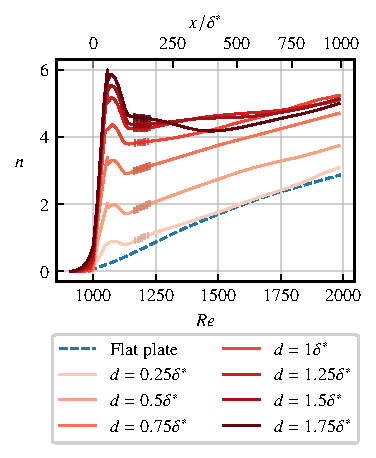
\includegraphics{Images/nfactorCurvesw40.pdf}
		\caption{Gaps with constant width $w=40\dstar$.}
		\label{fig:nfactorCurvesB}
	\end{subfigure}
	\caption{$n$-factor evolution curves along the streamwise direction for different gap configurations at $\Rey=1000$. Small markers indicate the streamwise locations used to compute the average $\Delta n$ values (see equation~\ref{eq:deltan}). The flat-plate reference case is shown as a dashed blue line and the BFS case is shown as a dashed-dotted orange line.}
	\label{fig:nfactorCurves}
\end{figure}
Figure~\ref{fig:nfactorCurves} shows the resulting $n(x)$ curves for selected gap configurations. In figure~\ref{fig:nfactorCurvesA}, the gap depth is fixed at $d/\dstar=1.5$ and the width is varied over $w/\dstar\in[10,50]$, while in figure~\ref{fig:nfactorCurvesB}, the gap width is fixed at $w/\dstar=40$ and the depth is varied over $d/\dstar\in[0.25,1.75]$. In all cases, the first step of the gap starts at $x=0$. The curves show a similar overall trend. Within the gap, $n$ increases rapidly and reaches a maximum before the downstream edge. A similar peak in $n$ was also observed experimentally by \citet{jeffGaps}. Downstream of the gap, $n$ decreases significantly before recovering a monotonic growth trend similar to that of the flat-plate reference, although with some streamwise variation in slope.

For the constant-depth cases in figure~\ref{fig:nfactorCurvesA}, the BFS result is also included for reference. The BFS produces the largest amplification, with the gap results approaching this value as the gap width increases, in agreement with the predictions of \citet{jeffGaps}. Moreover, due to the absence of a second step, the BFS shows a smoother $n$-factor profile than the gap cases. The absence of the second step also means that the abrupt drop observed in the gap cases is not present in the BFS curve, but a more gradual decrease is observed instead. The differences in the subsequent recovery of the $n$ curves after the initial drop are less clear. This is particularly evident in figure~\ref{fig:nfactorCurvesB}, where the deeper gaps $(d/\dstar\geq1.5)$ recover more slowly than the shallower gaps, resulting in intersections between some of the curves. To investigate the origin of these trends, a local spatial stability analysis was performed using the equilibrium base flows and the parallel-flow assumption, $\boldsymbol{U}=(U(y),0)$. Under these conditions, solutions of the linearized equations are represented by modes of the form
\begin{equation}
	v'(x,y,t) = \hat{v}(y) \exp\left( \mathrm{i}(\alpha x - \omega t) \right),
\end{equation}
where $\alpha=\alpha_r+\mathrm{i}\alpha_i$ and $\omega=\omega_r+\mathrm{i}\omega_i$ are the complex streamwise wavenumber and temporal frequency, respectively, with $\alpha_r, \alpha_i,\omega_r,\omega_i\in\mathbb{R}$. In the temporal formulation, $\alpha=\alpha_r$ is real and $\omega$ is unknown. Under these assumptions, the linearized equations reduce to solving the following eigenvalue problem for $(\omega,\hat{v})$ (Orr--Sommerfeld problem) \citep{schmid2001stability}
\begin{equation}
	\big(\mathrm{D}^2-\alpha_r^2\big)^2\hat{v}
	-\mathrm{i}\Rey\left[
		(\alpha_r U-\omega)\big(\mathrm{D}^2-\alpha_r^2\big)
		-\alpha_r U''\right]\hat{v}=0,
\end{equation}
where $\mathrm{D}\equiv\mathrm{d}/\mathrm{d}y$. The real part of $\omega$, $\omega_r$, is the temporal frequency of the mode, while the imaginary part, $\omega_i$, is the temporal growth rate. For the cases considered here, the temporal growth rates are converted to spatial growth rates using Gaster's transformation \citep{gaster1962,gasterMath}. This gives the spatial amplification rate $\alpha_i$ required to determine the local spatial stability boundaries. The base flow profiles are extracted at discrete streamwise locations, excluding the immediate vicinity of the gap corners, where the parallel-flow approximation is not valid. At each $x$ location, the spatial growth rates are evaluated over the relevant frequency range. The frequency is then is nondimensionalized as
$
	F = 10^6\omega_r\nu / u_\infty^2
$
\citep{schmid2001stability}, and the frequencies corresponding to $\alpha_i=0$ are retained to create the neutral stability boundaries. Figure~\ref{fig:neutralcurves} shows the resulting neutral stability boundaries in the $(x/\dstar,F)$ plane for selected gap configurations, together with the flat-plate Blasius reference. The corresponding $\Rey$ values based on the displacement thickness are also indicated on a secondary axis for comparison with the literature.

\begin{figure}[ht]
	\centering
	\begin{subfigure}{0.495\linewidth}
		\centering
		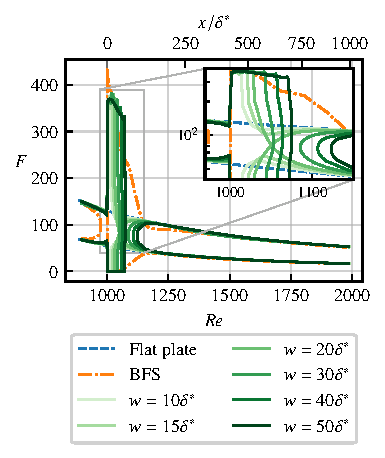
\includegraphics{Images/neutrald1.5.pdf}
		\caption{Gaps with constant depth $d=1.5\dstar$.}
	\end{subfigure}
	\begin{subfigure}{0.495\linewidth}
		\centering
		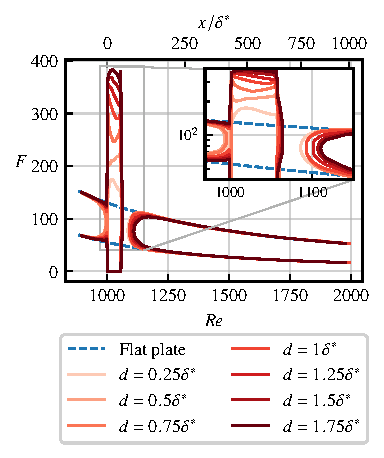
\includegraphics{Images/neutralw40.pdf}
		\caption{Gaps with constant width $w=40\dstar$.}
	\end{subfigure}
	\caption{Neutral curves ($-\alpha_i = 0$) of the spatial stability problem for (a) constant gap depth $d=1.5\dstar$ with varying width $w/\dstar$, and (b) constant gap width $w=40\dstar$ with varying depth $d/\dstar$, compared with the flat-plate reference flow.}
	\label{fig:neutralcurves}
\end{figure}

Several features of the local stability characteristics help explain the observed behaviour of $n$ in figure~\ref{fig:nfactorCurves}. Within the cavity, the unstable frequency range becomes broader. Since the system is forced with white noise, a wider range of frequencies is excited, resulting in faster growth of the perturbations. This leads to the enhanced amplification observed in the $n$-factor curves.

Downstream of small gaps, such as $(w/\dstar,d/\dstar)=(10,1.5)$ and $(w/\dstar,d/\dstar)=(15,1.5)$, the unstable region gradually approaches the flat-plate neutral boundary, and the $n$ curves recover towards the flat-plate reference. However, because the frequencies are excited differently within the cavity, and the problem being intrinsically advective, the downstream evolution does not necessarily have to follow the same monotonic growth as in the flat-plate case. Thus, even when the local stability boundaries agree closely with the flat-plate case at $x/\dstar\gg w$, the RMS of the perturbation field does not immediately return to the flat-plate counterpart.

For wider gaps, the unstable region develops two distinct branches separated by a locally stable frequency range. This locally stable region corresponds to the temporary and abrupt reduction in $n$ observed downstream of the wide gaps in figure~\ref{fig:nfactorCurves}. It also explains the slower recovery of the wider and deeper gaps shown in figure~\ref{fig:nfactorCurvesB} as the stable frequency range broadens with increasing gap width and depth.

To measure the gap-induced amplification of TS waves, \citet{jeffGaps} introduced the metric $\Delta N$ as follows: they first computed numerically the $n$-factor curves for the flat-plate reference flow, $n_\text{flat}(x)$, and they measured experimentally the transition location $x_\text{flat}^\text{trans}$ in the wind tunnel for the smooth plate configuration. Then, for each gap configuration considered, they measured the transition location $x_\text{gap}^\text{trans}$ and defined $\Delta N$ as the difference between the $n$-factor values of $n_\text{flat}(x_\text{flat}^\text{trans})$ and $n_\text{flat}(x_\text{gap}^\text{trans})$, i.e. 
\begin{equation}
	\Delta N := n_\text{flat}\big(x_\text{flat}^\text{trans}\big) - n_\text{flat}\big(x_\text{gap}^\text{trans}\big).
\end{equation}

In the present numerical framework, the transition location cannot be measured because the governing equations are linear. Thus, a new metric $\Delta n$ is introduced to quantify the gap-induced amplification of TS waves. $\Delta n$ is defined as an averaged difference between the $n$-factor curve for a given gap configuration and the flat-plate reference flow, i.e.
\begin{equation}\label{eq:deltan}
	\Delta n :=\frac{1}{|\mathcal{X}|}\int_{\mathcal{X}} \left(n_\text{gap}(x)-n_\text{flat}(x)\right)\mathrm{d}x,
\end{equation}
where $\mathcal{X}$ is a streamwise interval located downstream of the gap and $|\mathcal{X}|$ is its length. A $50\dstar$-long streamwise interval located downstream of the initial amplitude recovery zone (see small dashed markers on top of each amplification curve in figure~\ref{fig:nfactorCurves}) is chosen for $\mathcal{X}$. Within this region the direct effects of the gap and the associated non-parallel flow have decayed. Figure~\ref{fig:nfactorsketch} illustrates the differences between the two metrics $\Delta N$ and $\Delta n$. 

\begin{figure}[ht]
  \centering
	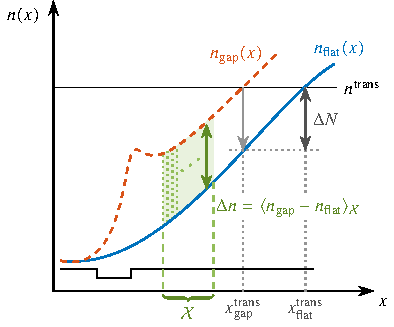
\includegraphics{Images/amplificationQualititiveNfactor.pdf}
	\caption{Schematic representation of way the two metrics $\Delta N$ and $\Delta n$ are computed. Subscripts \textit{flat} and \textit{gap} refer to the flat-plate reference flow and the flow over a generic gap, respectively. The superscript \textit{trans} indicates the abstract transition location.}
	\label{fig:nfactorsketch}
\end{figure}
The metric $\Delta n$ is evaluated for all parameter configurations that admit a stable steady base flow. To obtain a continuous representation over the stable parameter domain, the computed values are interpolated using Gaussian process regression with a Matérn kernel. Figure~\ref{fig:nfactorcountour} compares the resulting numerical contours (solid blue lines) with the experimental isolines $\Delta N=1,2,3,4,5$ reported by \citet{jeffGaps} (dashed orange lines).

\begin{figure}[ht]
	\centering
	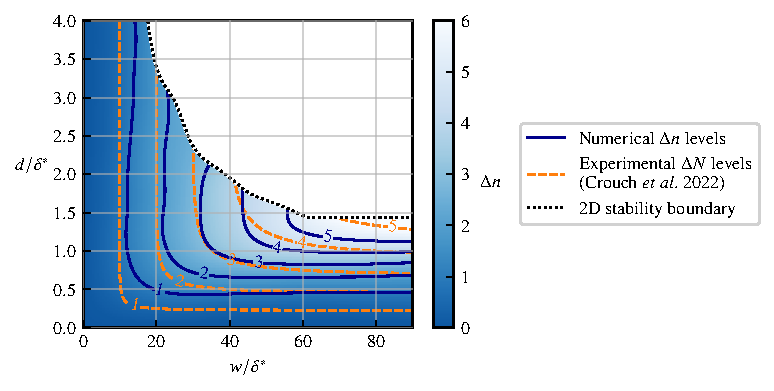
\includegraphics{Images/DeltaNcountour.pdf}
	\caption{Contour map of $\Delta n$ on the stable side of the parameter grid $(w/\dstar,d/\dstar)\in[0,90]\times[0,4]$. Dark blue solid contours indicate the corresponding numerical predictions. Orange dashed contours indicate experimental levels from \citet{jeffGaps} for $\Delta N=1,2,3,4, 5$.}\label{fig:nfactorcountour}
\end{figure}
The agreement with the numerically-computed countours of $\Delta n$ and the experimentally computed countours of $\Delta N$ is good. Both characteristic trends are reproduced: for narrow gaps ($w/\dstar\lesssim20$), the isolines are predominantly vertical, where the amplification is primarily determined by the gap width; for shallow gaps ($d/\dstar\lesssim1.5$), the isolines are predominantly horizontal, where the amplification is primarily determined by the gap depth. There is, however, a slight mismatch at higher $\Delta n$ values, where the numerical predictions overestimate the experimental $\Delta N$ results. There are several possible reasons for this difference.

Although the TS-wave convective instability mechanism is two-dimensional, \citet{jeffGaps} conducted their experiments in a three-dimensional wind tunnel at low Mach number. In contrast, the present simulations use a two-dimensional domain and solve the incompressible Navier--Stokes equations. This difference in dimensionality may contribute to the observed discrepancies, while the incompressibility assumption may also play a role. In addition, the choice of the averaging interval $\mathcal{X}$ in \eqref{eq:deltan} introduces a small, but non-negligible effect on the resulting $\Delta n$ values, particularly for gaps with large amplification, due to the streamwise variation of the $n$ curves.

To extend the analysis and study the effect of Reynolds number on TS-wave amplification, it is necessary to understand how the linear stability boundary changes with $\Rey$. The dependence of the supercritical Hopf bifurcation on Reynolds number is shown in figure~\ref{fig:2DdynamicsRe} for $\Rey\in[800,3000]$. Increasing $\Rey$ shifts the Hopf stability boundary towards smaller gap dimensions. As $w/\dstar$ increases along the curves, the stability boundary approaches the limiting behaviour associated with an isolated FFS, which is inherently more unstable than a BFS \citep{lanzerstorferBFS,lanzerstorferFFS}. At $\Rey=1000$, the onset of global instability is found at $d/\dstar\in(2.75,3.0)$ for the FFS and at $d/\dstar\in(3,3.25)$ for the backward-facing step.

\begin{figure}[ht]
	\centering
	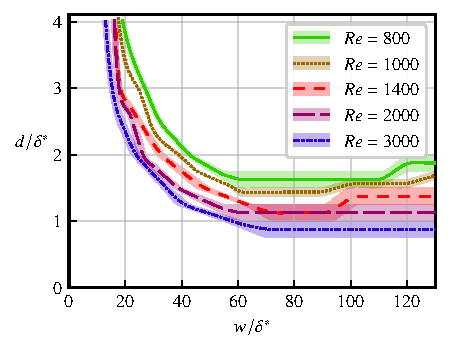
\includegraphics{Images/hopfBifReynolds.pdf}
	\caption{Linear stability boundaries in the $(w/\dstar, d/\dstar)$ plane for $\Rey \in [800, 3000]$. Shaded bands indicate the uncertainty associated with interpolation between the discrete simulation points.}
	\label{fig:2DdynamicsRe}
\end{figure}
The Reynolds-number dependence of TS-wave amplification is further illustrated in figure~\ref{fig:nfactorcountourRe} for two particular Reynolds number: $\Rey=800$ and $\Rey=3000$. Increasing the Reynolds number increases the amplification associated with a given gap geometry, shifting the $\Delta n$ contours towards smaller gap dimensions. At $\Rey=800$, relatively large gaps are required to produce $\Delta n\approx3$. At $\Rey=3000$, by contrast, even relatively shallow or narrow gaps, such as $w/\dstar\approx20$ and $d/\dstar\approx1$, can produce $\Delta n>4$. The stronger TS-wave amplification at higher Reynolds number is consistent with the corresponding shift of the Hopf boundary towards smaller gap dimensions.

\begin{figure}[ht]
	\centering
	\begin{subfigure}{0.497\linewidth}
		\centering
		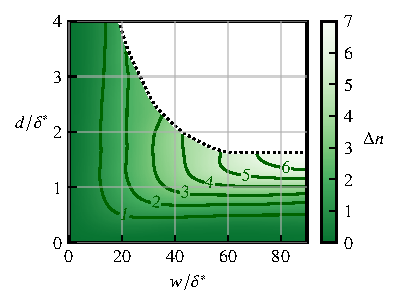
\includegraphics{Images/DeltaNcountourOnlyNumericRe800.pdf}
		\caption{$\Rey=800$}
	\end{subfigure}
	\begin{subfigure}{0.497\linewidth}
		\centering
		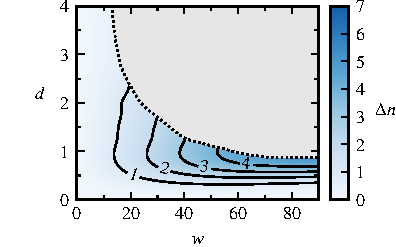
\includegraphics{Images/DeltaNcountourOnlyNumericRe3000.pdf}
		\caption{$\Rey=3000$}
	\end{subfigure}
	\caption{Contour maps of numerical predictions of $\Delta n$ over the stable parameter space $(w/\dstar,d/\dstar) \in [0,90] \times [0,4]$ for (a) $\Rey=800$ and (b) $\Rey=3000$.}
	\label{fig:nfactorcountourRe}
\end{figure}

\subsection{Limit cycles (2D unstable regime)}\label{sec:bifurcations}
As the gap width or depth is increased the flow undergoes supercritical Hopf bifurcation (green line in figure~\ref{fig:2Ddynamics1000}). The supercritical nature of the Hopf bifurcation is confirmed by the crossing of a single complex-conjugate pair of eigenvalues through the imaginary axis, while the remaining eigenvalues retain negative real parts. The expected normal-form scaling is further verified by tracking the amplitude of the emerging limit cycle along two continuation paths crossing the Hopf boundary in the $(w/\dstar,d/\dstar)$ parameter plane. One path crosses the boundary by varying the gap width at fixed depth, while the other crosses it along an oblique direction in parameter space. Denoting the distance from the bifurcation point along either path by the scalar parameter $\mu$, with $\mu=0$ at the Hopf boundary and $\mu>0$ on the unstable side of the equilibrium, the normal form for a supercritical Hopf bifurcation predicts
\begin{equation}
	A(\mu)\propto\sqrt{\mu}.
\end{equation}
where $A$ is an appropriate measure of the limit-cycle amplitude. Figure~\ref{fig:hopfAmplitude} shows the squared $L^2$ norm of the perturbation wall-normal velocity, $\boldsymbol{u}'=\boldsymbol{u}-\boldsymbol{U}$, as a function of $\mu$ along the two paths. The approximately linear dependence of $A^2$ on $\mu$ agrees with the expected square-root scaling of the limit-cycle amplitude.

\begin{figure}[ht]
	\centering
	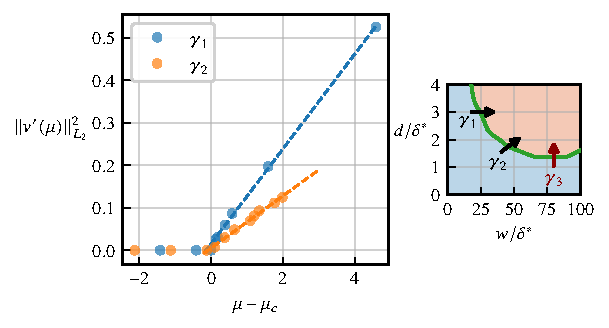
\includegraphics{Images/hopfAmplitude.pdf}
	\caption{Amplitude evolution of the limit cycle for different crossing locations of the Hopf bifurcation in the $(w/\dstar, d/\dstar)$ parameter plane. The two continuation paths are indicated in the small plot in the right.}
	\label{fig:hopfAmplitude}
\end{figure}
Although a single complex-conjugate pair of eigenvalues also crosses the imaginary axis for shallow gaps ($w/\dstar \gtrsim 75$ and $d/\dstar \sim 1.5$; $\boldsymbol{\gamma}_3$ path in figure~\ref{fig:hopfAmplitude}), the squared perturbation amplitude does not exhibit the expected linear dependence on $\mu$. In this shallow-gap regime, the frequency of the most unstable eigenmode approaches the neutral stability boundary of local stability analysis, and the resulting instability becomes increasingly influenced by the spatial growth of the mode. Consequently, its amplitude is not determined solely by the distance from the bifurcation point. Figure~\ref{fig:L2normPO} shows the evolution of the wall-normal $L^2$ norm of the perturbation velocity along the streamwise direction for different gap configurations. In the figure, the origin $x$ coordinate refers to the end of all the gaps considered. As mentioned above, the limit cycles are localized near the downstream edge of the gap. It can be seen that for the configurations $w=60\dstar$ and $w=63\dstar$, the $L^2$ amplitude considered decays quickly downstream of the gap. As the gap width is increased ($w=65\dstar$), the amplitude has a transient growth region downstream of the gap, which indicates that in a particular region of the domain, the frequency of the limit cycle lies just inside the unstable region of the LSA. Increasing the gap width further ($w\geq 70\dstar$), the limit cycle frequency completely lies within the unstable region of the LSA and the two mechanisms of instability (global and convective) reinforce each other, leading to a completed destabilized boundary layer.

\begin{figure}[ht]
	\centering
	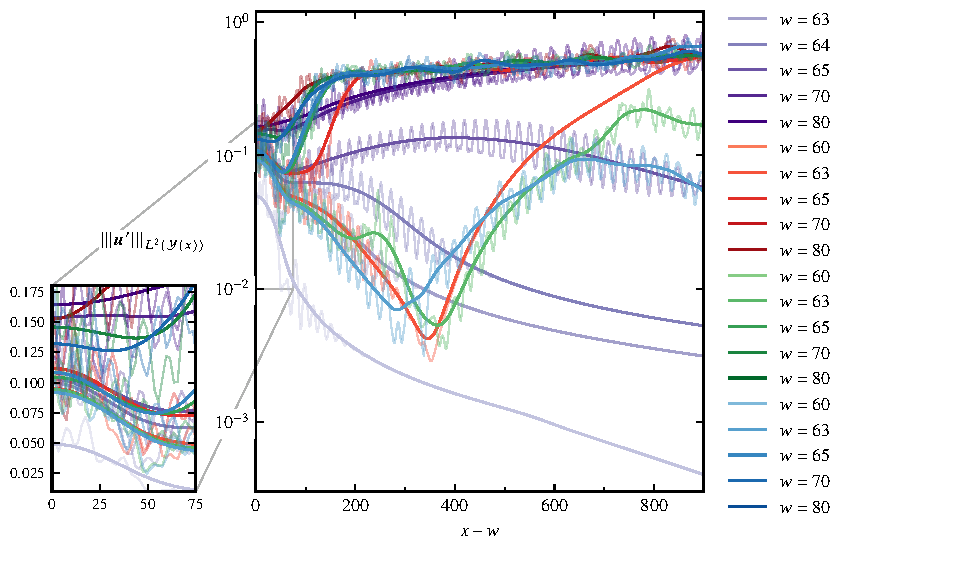
\includegraphics{Images/L2POvsX.pdf}
	\caption{Streamwise distribution of the wall-normal $L^2$ norm of the magnitude of the perturbation velocity, ${\||\boldsymbol{u}'|\|}_{L^2(\mathcal{Y}(x))}$, for different gap configurations of variable widths at fixed gap depth $d=1.5\dstar$ and $\Rey=1000$. Temporal averaging is performed to obtain the smooth curves, while the low-opacity curves represent an instantaneous snapshot of the trajectories.}
	\label{fig:L2normPO}
\end{figure}

\begin{figure}[ht]
	\centering
	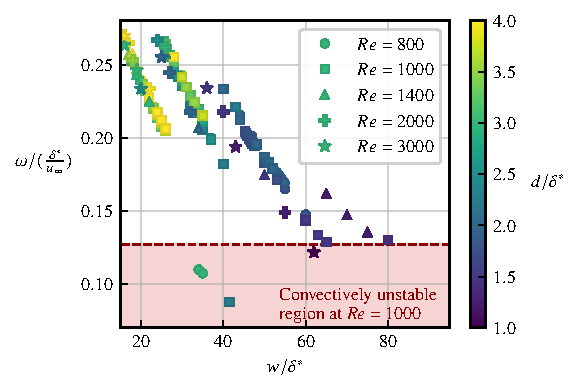
\includegraphics{Images/freqUnstableMode.pdf}
	\caption{Limit cycle frequencies as a function of gap width $w/\dstar$ for different gap depths and Reynolds numbers. Marker shading indicates gap depth, with darker markers corresponding to shallower gaps and lighter markers corresponding to deeper gaps,	and marker shape denotes Reynolds number. The red shaded region indicates the approximately constant frequency range of convectively unstable TS waves at the corresponding Reynolds number in the neighborhood of the gap.}
	\label{fig:freqUnstableMode}
\end{figure}
The fundamental frequency $\omega$ of the limit cycles varies with Reynolds number and cavity geometry, as summarized in figure~\ref{fig:freqUnstableMode}. For narrow gaps ($w/\dstar\lesssim60$), the frequencies form three distinct modal branches associated with the cavity geometry and recirculation dynamics. As the gap width increases at fixed depth, the dominant mode of the narrower cavity loses stability and a different periodic state emerges, with a frequency more representative of the larger cavity. The weaker interactions between branches observed across different depths indicate a secondary dependence on the gap geometry. For wide gaps ($w/\dstar\gtrsim65$), the limit-cycle frequencies approach the characteristic frequency range of convectively unstable TS waves at the corresponding Reynolds number. The associated modes have longer streamwise scales and lower frequencies.

Several isolated points around $w=40\dstar$ and $\omega/(\dstar/u_\infty)=0.1$ in figure~\ref{fig:freqUnstableMode} correspond to period-doubling bifurcations, providing a route from periodic to chaotic dynamics. Figure~\ref{fig:periodDoubling} illustrates one such bifurcation for two gap configurations at $\Rey=800$. Increasing the gap width from $w/\dstar=33$ to $33.5$ at $d/\dstar=3$ results in a limit cycle with approximately twice the period.

\begin{figure}[ht]
	\centering
	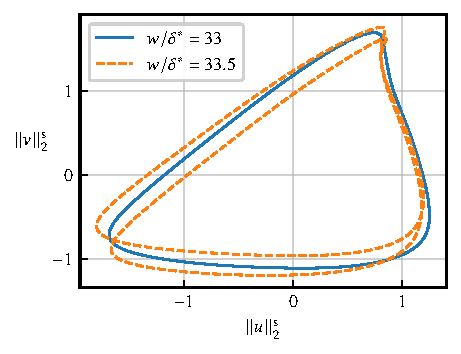
\includegraphics{Images/periodDoubling.pdf}
	\caption{Periodic orbits for the gap configurations $(w/\dstar, d/\dstar) = (33, 3)$ and $(w/\dstar, d/\dstar) = (33.5, 3)$ at $\Rey = 800$ projected onto the two dimensional space $(\|u\|_2^\text{s}, \|v\|_2^\text{s})$. Here $\|\cdot\|_2^\text{s}:=(\|\cdot\|_2-\overline{\|\cdot\|_2})/\sigma(\|\cdot\|_2)$ denotes the standardized $L^2$ norm over the computational domain, with $\sigma$ denoting the standard deviation of the corresponding time series.}
	\label{fig:periodDoubling}
\end{figure}
\section{Three-dimensional dynamics}\label{sec:3Ddynamics}
Even though the primary convective instabilities in the boundary layer are two-dimensional, global stability analysis (figure~\ref{fig:3d2dDynamics1000}) has showed that purely three-dimensional instabilities can arise before the two-dimensional instabilities if the gap is sufficiently deep. In this section, we investigate the nonlinear three-dimensional dynamics to be able to understand the different transition scenarios that can arise in the gapped laminar boundary layer.

In region II of figure~\ref{fig:3d2dDynamics1000}, a purely three-dimensional mode has positive growth rate. DNS has been carried out to investigate the nonlinear evolution of this mode. Initially, the flow grows in the direction of the three-dimensional eigenmode, and the amplitude of the three-dimensional mode grows exponentially. However, as the amplitude saturates, the boundary layer downstream of the gap remains stable.  

The three-dimensional instability becomes particularly important once the two-dimensional equilibrium has already lost stability. Increasing the gap width beyond the two-dimensional stability boundary leads to a chaotic attractor that develops predominantly near the downstream edge of the gap (figure~\ref{fig:3dtransAtGap}). For deep gaps ($d/\dstar\gtrsim2$), this behaviour corresponds to region III in figure~\ref{fig:3d2dDynamics1000}, whereas for shallow gaps ($d/\dstar\lesssim2$) it corresponds to region IV. In both cases, the two-dimensional periodic orbit that emerges after the Hopf bifurcation can become unstable to three-dimensional perturbations. A separate region, denoted region V, contains two-dimensional periodic orbits that remain stable to three-dimensional perturbations; an example is $(w/\dstar,d/\dstar)=(60,1.5)$.

\begin{figure}[ht]
	\centering
	\begin{subfigure}{0.49\linewidth}
		\centering
		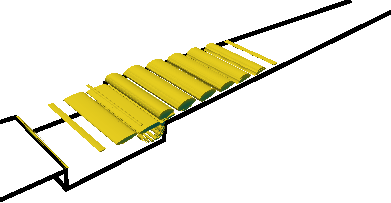
\includegraphics{Images/3DtransImages/pdfs/d4w19_3d_L2crit_10.pdf}
		\vspace{-1.0cm}
		\caption{$t=1677$}
		\label{fig:3dtransAtGap_a}
	\end{subfigure}
	\hfill
	\begin{subfigure}{0.49\linewidth}
		\centering
		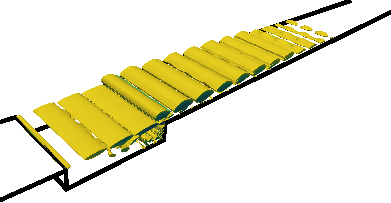
\includegraphics{Images/3DtransImages/pdfs/d4w19_3d_L2crit_12.pdf}
		\vspace{-1.0cm}
		\caption{$t=2277$}
		\label{fig:3dtransAtGap_b}
	\end{subfigure}\\
	\vspace{-1.0cm}
	\begin{subfigure}{0.49\linewidth}
		\centering
		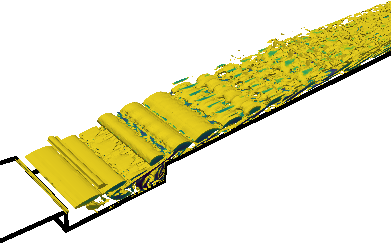
\includegraphics{Images/3DtransImages/pdfs/d4w19_3d_L2crit_14_big.pdf}
		\vspace{-1.0cm}
		\caption{$t=2797$}
		\label{fig:3dtransAtGap_c}
	\end{subfigure}
	\hfill
	\begin{subfigure}{0.49\linewidth}
		\centering
		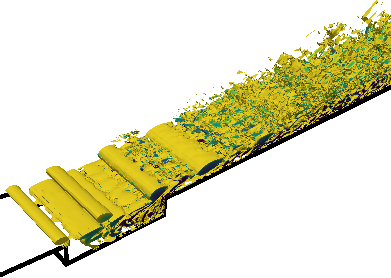
\includegraphics{Images/3DtransImages/pdfs/d4w19_3d_L2crit_17_big.pdf}
		\vspace{-1.0cm}
		\caption{$t=3677$}
		\label{fig:3dtransAtGap_d}
	\end{subfigure}\\
	\vspace{0.5cm}
	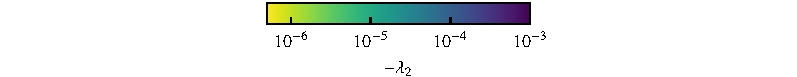
\includegraphics{Images/3DtransImages/pdfs/colorbar.pdf}
	\caption{Transition sequence for $w= 19\dstar$ and $d= 4\dstar$ at $\Rey = 1000$. Vortical structures are visualized using $\lambda_2$-criterion isosurfaces. The simulation time corresponding to each state is indicated next to each visualization.}
	\label{fig:3dtransAtGap}
\end{figure}
Figure~\ref{fig:3dtransAtGap} illustrates the transition sequence for the deep-gap configuration $(w/\dstar,d/\dstar)=(19,4)$ at $\Rey=1000$. The flow is initialized with a small perturbation in the direction of the most unstable two-dimensional mode (figure~\ref{fig:3dtransAtGap_a}). It first evolves towards the corresponding periodic orbit, which is unstable to three-dimensional perturbations. As the instability develops, three-dimensional structures appear both within the cavity and downstream of the gap (figure~\ref{fig:3dtransAtGap_b}). The flow, then, subsequently departs from the two-dimensional periodic orbit and develops a chaotic state in the downstream boundary layer (figure~\ref{fig:3dtransAtGap_c}). At the later stages, the downstream flow exhibits increasingly complex three-dimensional structures leading to fully developed turbulence (figure~\ref{fig:3dtransAtGap_d}). Nevertheless, in the immediate vicinity of the downstream gap edge, the characteristic frequency of the underlying two-dimensional oscillation remains present. This behaviour is consistent with the strong non-TS-wave spectral peak reported experimentally by \citet{jeffGaps}.

The transition sequence is not restricted to initial perturbations aligned with the most unstable two-dimensional mode. Since the growth rate of the three-dimensional mode is slightly larger than that of the two-dimensional mode, the flow can instead be initialized with a small perturbation in the direction of the most unstable three-dimensional mode. In this case, the three-dimensional disturbance initially follows the linear growth predicted by the unstable eigenmode. As its amplitude increases, nonlinear effects become important and the flow departs from the eigenmode direction, generating finite-amplitude three-dimensional structures that trigger the development and subsequent growth of the two-dimensional mode. The flow then evolves towards a chaotic state similar to that shown in figure~\ref{fig:3dtransAtGap}. These observations show that the three-dimensional instability can provide the perturbation pathway through which transition develops, but that the three-dimensional instability alone is insufficient to produce boundary-layer breakdown. Rather, the bypass mechanism is associated with the interaction between the three-dimensional instability and the two-dimensional oscillatory mode.

To further examine this interaction, a Floquet analysis is performed about the three-dimensionally unstable two-dimensional limit cycle. In contrast to the previous linear stability analysis, in which the base state is a steady equilibrium, the base state for the Floquet analysis is the periodic orbit, $\boldsymbol{U}_\text{floq}(t) = \boldsymbol{u}_\text{p.o.}(t)$, where $\boldsymbol{u}_\text{p.o.}$ denotes the two-dimensional periodic solution.

\begin{figure}[ht]
	\centering
	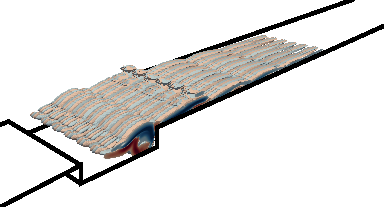
\includegraphics{Images/2D_3Dmode/pdfs/d4w19_3dFloquetmode.pdf}\\[0pt]
	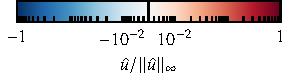
\includegraphics{Images/2D_3Dmode/pdfs/colorbar.pdf}
	\caption{Most unstable floquet mode for the gap configuration with $w=19\dstar$ and $d=4\dstar$ at $\Rey = 1000$. Isosurfaces of the streamwise velocity perturbation $u'$ are shown.}
	\label{fig:3dfloquetMode}
\end{figure}

Finally, region IV and V in figure~\ref{fig:3d2dDynamics1000} corresponds to configurations for which the two-dimensional instability occurs before the three-dimensional instability. The boundary separating regions III and IV, III and V and IV and V has not been resolved in detail. A representative shallow-gap transition in region IV is shown in figure~\ref{fig:3dtransShallowGap}. Unlike the deep-gap case, the transition is initiated by the two-dimensional instability and subsequently develops three-dimensional structure farther downstream.
\begin{figure}[ht]
	\centering
	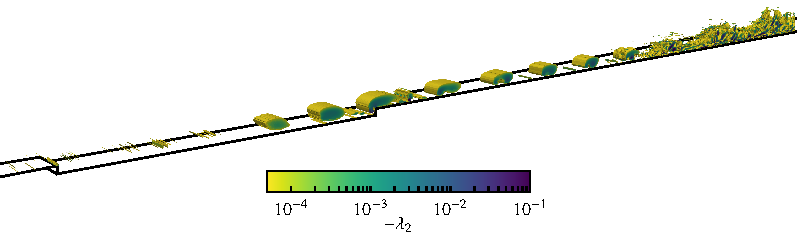
\includegraphics{Images/3DtransImages/pdfs/d1.5w80Lz5_3d_L2crit_31.pdf}
	\caption{Transition scenario for a gap configuration with $w=80\dstar$ and $d=1.5\dstar$ at $\Rey = 1000$. Vortical structures are visualized using $\lambda_2$-criterion isosurfaces.}
	\label{fig:3dtransShallowGap}
\end{figure}

\section{Conclusions}\label{sec:conclusions}

The effect of a spanwise-uniform rectangular surface gap on the stability and transition of a laminar incompressible boundary layer has been investigated by direct numerical simulation and global stability analysis, over the parameter range $w/\dstar\in(0,130]$, $d/\dstar\in(0,4]$ and $\Rey_\dstar\in[800,3000]$. Rather than treating the gap solely as a modifier of Tollmien--Schlichting (TS) amplification, we have characterised it as a dynamical system and followed the sequence of bifurcations through which it loses stability. The main findings are as follows.

First, the long-time two-dimensional dynamics of the gap flow fall into three classes: equilibria, limit cycles and chaotic attractors. The equilibrium topology inside the cavity is governed by the aspect ratio $w/d$ and reproduces the open-to-closed cavity sequence, from a single recirculation beneath a bridging shear layer at small $w/d$, through an elongated shallow recirculation, to a reattaching, closed configuration at large $w/d$ that approaches the superposition of an isolated backward- and forward-facing step \citep{Zhang2005,Crook2013}. The equilibrium loses stability through a supercritical Hopf bifurcation: a single complex-conjugate pair crosses the imaginary axis and the emerging limit-cycle amplitude follows the normal-form scaling $A\propto\sqrt{\mu}$ along continuation paths crossing the boundary in the $(w/\dstar,d/\dstar)$ plane. The resulting oscillation is localised at the downstream gap edge. Further increases in gap width produce period-doubling bifurcations and, ultimately, two-dimensional chaos. The neutral curve itself is non-monotonic in depth: the critical width first increases, peaking where the interference between the two edges is strongest, and then decreases towards the isolated-step limit, in which the forward-facing step is the more unstable of the two \citep{lanzerstorferBFS,lanzerstorferFFS}. Increasing the Reynolds number shifts the entire boundary towards smaller gap dimensions.

Second, wherever a stable equilibrium exists, the gap-induced amplification of TS waves is well described by the increment $\Delta n$ obtained from stochastically forced linearised simulations. The computed contours reproduce the two limiting behaviours measured by \citet{jeffGaps}: for narrow gaps the isolines are essentially vertical, so that the amplification is set by the width, while for shallow gaps they are essentially horizontal, so that it is set by the depth, with the backward-facing step recovered as the wide-gap limit. The agreement is obtained without any fitted correlation, and the residual overprediction at large $\Delta n$ is consistent with the two-dimensional, incompressible idealisation adopted here and with the sensitivity of the averaged metric to the streamwise window over which it is evaluated. Local spatial stability analysis of the equilibrium profiles explains both trends. Inside the cavity the band of unstable frequencies broadens, so that broadband forcing is amplified over a wider spectrum and $n$ peaks before the downstream edge, as also observed experimentally. Downstream of wide and deep gaps the unstable region splits into two branches separated by a locally stable frequency window, which accounts for the abrupt drop in $n$ immediately after the gap and for the slower recovery of the deeper configurations. Increasing the Reynolds number increases $\Delta n$ for a fixed geometry, consistently with the corresponding displacement of the Hopf boundary.

Third, and centrally, the transition scenario at the gap is not governed by the linear global instability of the steady flow. For deep gaps, $d/\dstar\gtrsim1.75$, the purely three-dimensional boundary lies at smaller widths than the two-dimensional one, so that spanwise-periodic perturbations destabilise the equilibrium first; the corresponding mode produces long streamwise streaks downstream of the gap at a frequency roughly an order of magnitude below that of the two-dimensional mode. Direct simulation shows, however, that this instability saturates into a finite-amplitude state that leaves the downstream boundary layer laminar. Breakdown requires instead a two-dimensional periodic orbit that is itself unstable to three-dimensional perturbations. When such an orbit exists, the flow departs from it, develops three-dimensional chaotic motion downstream of the gap and proceeds to fully developed turbulence, while retaining the frequency of the underlying two-dimensional oscillation in the immediate vicinity of the downstream edge --- consistent with the strong non-TS spectral peak reported in the experiments. The same end state is reached when the flow is initialised along the three-dimensional eigenmode, which then acts as the perturbation pathway that triggers the two-dimensional oscillation rather than as the instability responsible for breakdown. The existence of a three-dimensionally unstable two-dimensional periodic orbit is thus both necessary and sufficient for transition at the gap, and the composite boundary constructed from the two- and three-dimensional stability curves reproduces the experimental bypass boundary of \citet{jeffGaps} over the full range considered. Configurations were also identified, at shallow depths, in which a two-dimensional limit cycle remains stable to spanwise perturbations; these do not transition at the gap.

Taken together, these results give a single, mechanistically grounded picture of gap effects on transition. A gap whose equilibrium is stable acts as a passive distortion that modifies the amplification of an instability it does not create; its effect is completely characterised by $\Delta n$, and the variable-$N$ framework \citep{crouchKosoryginNg2006,crouch2021predicting} applies. A gap large enough to have crossed the Hopf boundary and to possess a three-dimensionally unstable periodic orbit is an active oscillator that manufactures its own disturbances; for such a gap the notion of a modified critical $N$-factor is meaningless, because transition no longer occurs through the amplification of incoming TS waves. The boundary between the two regimes is not an empirical threshold but a bifurcation, and it can be computed directly from the flow.

Two practical implications follow. Since global instability of the equilibrium can precede the appearance of a three-dimensionally unstable periodic orbit, the onset of global instability is a conservative but not a sharp criterion for transition at the gap; using it alone would penalise geometries that remain laminar. Conversely, because the Hopf boundary moves towards smaller gaps as the Reynolds number increases, tolerances calibrated at one flight condition cannot be transferred unchanged to another.

Several limitations delimit the scope of these conclusions and indicate natural extensions. The analysis is incompressible, whereas the acoustic feedback invoked to explain the non-monotonic depth dependence observed for deep gaps in compressible flow \citep{zahnRist,rossiter1964} is necessarily absent here; a compressible study would establish whether that mechanism modifies the bifurcation sequence or merely shifts its boundaries. The gap is spanwise-uniform and the external flow has zero pressure gradient, while the experiments of \citet{jeffGaps} were conducted under a mild adverse gradient, and \citet{beguetONERA} identified pressure gradient as a factor requiring further investigation. Finally, the present configuration is nominally two-dimensional; on swept surfaces the primary instability is crossflow rather than TS \citep{3dBoundaryLayers}, and the interaction of a gap with crossflow modes, as already documented for steps \citep{eppink2019,tufts2017}, remains open. The methodology developed here --- classifying the attractors of the excrescence flow and testing their three-dimensional stability --- is not specific to gaps, and should transfer directly to these cases.

\bibliographystyle{jfm}
\bibliography{jfm}

\end{document}
